% This file should be rename with the speaker's last name. (e.g : smith)

% Write the author names in the order you wish them to appear
% and underline the one who will give the talk.

% Only the speaker's email address is required.

\begin{abstract_online}{DGS assisted activities around \\ \quad \\ the Golden Ratio in Space and Time}{%
        \underline{Thierry Dana-Picard}$^{1}$, Sara Hershkovitz$^{2}$}{[ndp@jct.ac.il]
        }{%
        $^1$ Department of Mathematics, Jerusalem College of Technology, Jerusalem, Israel \newline{}$^2$ Center for Educational Technology, Tel Aviv, Israel \newline{}}

Mario Livio [4] wrote that "The history of art shows that in the long search for an elusive canon or “perfect” proportion, one that would somehow automatically confer aesthetically pleasing qualities on all works of art, the Golden Ratio has proven to be the most enduring". This Golden Ratio is defined as follows.

Consider a segment $AB$ and a point $C$ on this segment, as in Figure ~\ref{golden ratio def}.

\begin{figure}[h]
\centering
\mbox{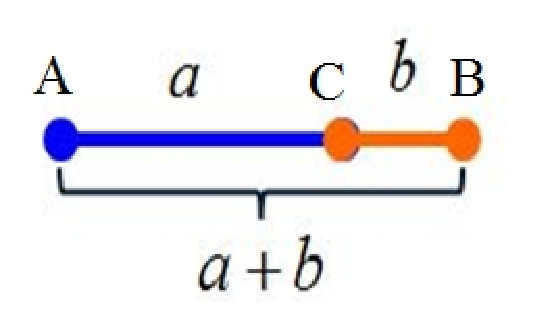
\epsfig{file=golden_ratio-definition.eps,height=2cm}}
\caption{Harmonious divide of a segment}
\label{golden ratio def}
\end{figure}
Denote $a=AC$ and $b=CB$. Then the division of the segment is made according to the Golden Ratio if
\begin{equation*}
\frac{a+b}{a}=\frac{a}{b}.
\end{equation*}
It is easily shown that this ratio is equal to  $\frac{1+\sqrt{5}}{2}$, and is denoted by the Greek letter $\phi$.
Traditionally, the ancien Greeks are credited for this choice. Koshy [5] writes that the letter $\phi$ has been chosen in honor of the sculptor Phidias by the American Mathematician Mark Barr. In Chapters 20-21, Koshy mentions other reasons for the choice of this Greek letter. He refers to Coxeter for an explanation why this number has been also denoted by the Greek letter $\tau$, the first letter of the Greek word $\tau o \mu \eta$ (section).

Actually, there are occurrences of the Golden Ratio in more ancient sources. It appears in the Bible, and recently, ancient jewelry and objects related to observation of planets have been discovered in chalcolithic archeological sites near Varna, Bulgaria.
Activities around the Golden Section may be developed for every age of students. For each category of students, technology may be used. Among them:
\begin{enumerate}
\item The geometry of plane configurations, leading to the study of specific buildings. We will show the Golden Ration appearing in an Italian octagonal Middle Ages castle and in a $19^{th}$ century synagogue in Budapest, Hungary. The experiments have been made using GeoGebra\footnote{\url{https://www.geogebra.org/}}, a free downloadable Dynamical Geometry System (DGS). This is a good opportunity to apply a specific feature of GeoGebra for augmented reality.
\item The Golden Ratio appears also when studying the graphs of trigonometric functions and their tangents; see Figure ~\ref{fig trig}. This can be studied using a CAS.
 \begin{figure}[h]
\centering
\mbox{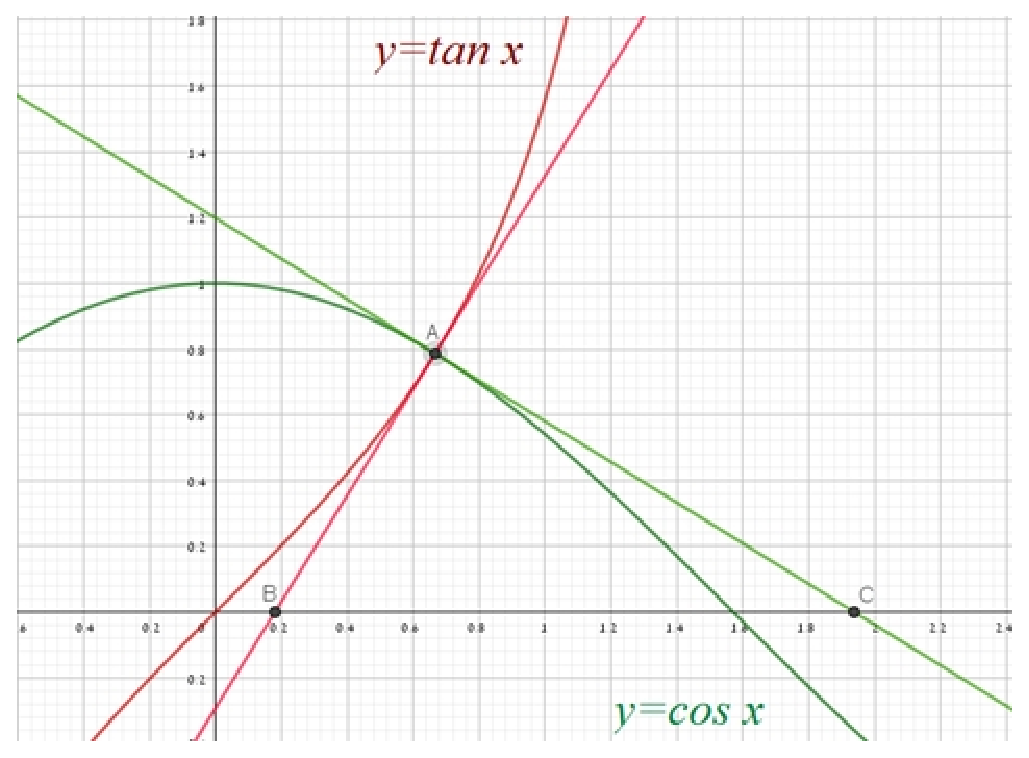
\epsfig{file=golden_ratio-trigo.eps,height=3.5cm}}
\caption{Tangents to the graphs of trigonometric functions}
\label{fig trig}
\end{figure}
\item The determination of the center of mass of earrings made when cutting off a disk form another disk, in a certain configuration. In this case, double integrals have to be computed. A Computer Algebra System has been used.
\item In music, a non-geometric setting, specific accords are determined by frequency ratios equal to specific ratio of Fibonacci numbers. This can be checked using a CAS. Of course of full experiment would requires other kinds of technology, available in an acoustic lab.
\item Geometry and acoustics may be connected with a study of the shapes of various instruments. This study may be performed using a DGS.
\item The needed computations for the traditional Hebrew calendar, which is lunar-solar\footnote{Unlike the Gregorian calendar, which is purely solar, and unlike the Muslim calendar, which is purely lunar.} are based on the so-called Meton formula. This formula reads: $12 \cdot 12 + 7 \cdot 13 =235$. Actually, the number of days in 235 lunations is equal to the number of days in 19 tropical years. In order for the High Holidays to be in phase with the seasons, the Hebrew calendar is organized in cycles of 19 years, where 12 years are regular (12 months each) and 7 of them are 13-month years. This also leads to the appearance of the Golden Ratio in a non-geometric setting. It must be noted that, as the interval between two consecutive new moons is not an integer, neither is the number of days in a tropical year, Meton formula is not enough for establishing a calendar. Historically, these computations have been made by hand, but technology makes them easier.
\end{enumerate}
For some of these examples, we will present technology based activities which have been proposed to students of various ages, some of them undergraduates, but the last one with K5 students.


\textbf{Keywords} \newline{} Golden Ratio, DGS, CAS

\textbf{References} \newline{}
[1] \textsc{Th. Dana-Picard; S. Hershkovitz}, A Glimpse at Mathematics in Jewish Traditional Artefacts, \emph{Symmetry: Culture and Science}, \textbf{29}(2), 307-317 (2018).\newline{}
[2] \textsc{Th. Dana-Picard; S. Hershkovitz}, Geometrical Features of a Jewish Monument: Study with a DGS. To appear in \emph{the Journal of the Mathematics and the Arts} (2019). \newline{}
[3] \textsc{Th. Dana-Picard}, \emph{Rabbits, beauty and kindness – on mathematics and aesthetics: the hidden hand in nature}, in \emph(TDP and G. Morali, edts) Ladaat Baarets Darekkha Vol. I , JCT and Bet-El Library Publishers, 69-96 (2017). In Hebrew.\newline{}
[4] \textsc{M. Livio}, \emph{, The Golden Ratio: The Story of Phi, the World’s Most Astonishing Number}. Broadway Books, New York, 2002. \newline{}
[5] \textsc{Th. Koshy}. \emph{Fibonacci and Lucas Numbers with Applications}, J. Wiley, New York, 2001.
\end{abstract_online}




